\section{Control}
En la Figura~\ref{fig:diagrama-de-robot-industrial}. se muestra el diagrama de bloques correspondiente al sistema de control de un robot industrial. Este diagrama describe el flujo de información desde la entrada del usuario hasta el movimiento del robot, incluyendo el control, la planificación de trayectoria y el modelo dinámico.

\begin{itemize}
	\item \textbf{Valores definidos por el usuario:} Se introducen parámetros como puntos coordenados, velocidad mínima, aceleración mínima y tipo de trayectoria. Estos definen el objetivo deseado para el efector final del robot.
	
	\item \textbf{Planificación de trayectoria:} Genera valores deseados para el efector final (posición, velocidad, aceleración) en el espacio cartesiano. Estos valores permiten un movimiento suave y seguro del robot.
	
	\item \textbf{Cinemática inversa:} Convierte los valores del efector final a coordenadas articulares (posición $q$, velocidad $\dot{q}$ y aceleración $\ddot{q}$), ya que el robot opera en este espacio.
	
	\item \textbf{Controlador:} Calcula el error entre la trayectoria deseada ($Z_d$) y la trayectoria real ($\hat{Z}$), y genera las señales de control necesarias (fuerza lineal o torque rotacional) para corregirlo.
	
	\item \textbf{Dinámica del robot:} Representa el modelo físico del robot, que puede ser no lineal ($\dot{x} = f(x, u)$) o

 \autoref{fig:diagrama-de-robot-industrial}.

\begin{figure}[h]
	\centering
	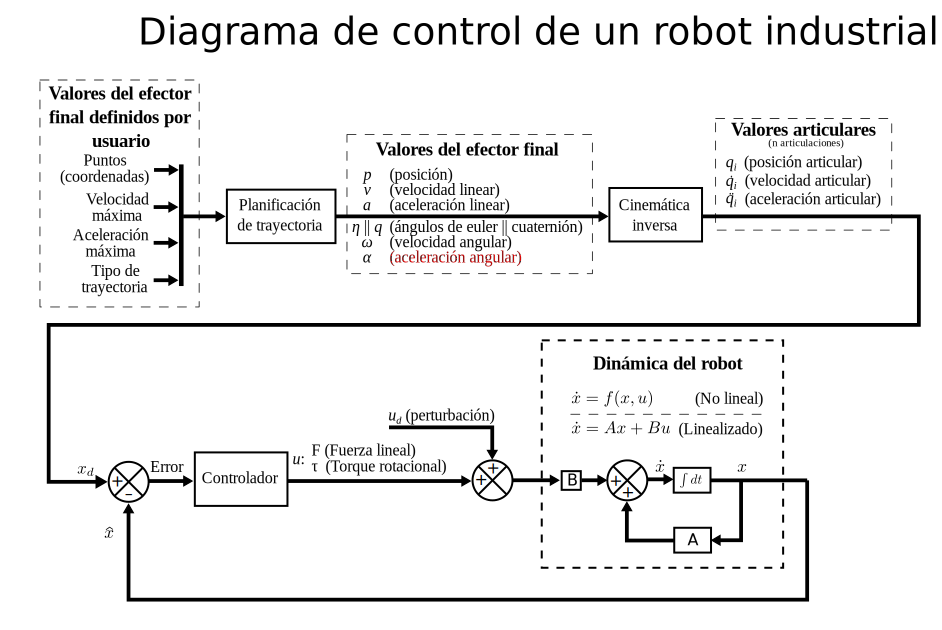
\includegraphics[width=\linewidth]{img/Diagrama_robot_industrial}
	\caption{Diagrama de bloques de un robot industrial}
	\label{fig:diagrama-de-robot-industrial}
\end{figure}
